\documentclass{article}

\usepackage{fancyhdr}
\usepackage{extramarks}
\usepackage{amsmath}
\usepackage{amsthm}
\usepackage{amsfonts}
\usepackage{tikz}
\usepackage[plain]{algorithm}
\usepackage{algpseudocode}
\usepackage{graphicx}
\usepackage{xcolor}
\usepackage[dvipsnames]{xcolor}

\usetikzlibrary{automata,positioning}

%
% Basic Document Settings
%

\topmargin=-0.45in
\evensidemargin=0in
\oddsidemargin=0in
\textwidth=6.5in
\textheight=9.0in
\headsep=0.25in

\linespread{1.1}

\pagestyle{fancy}
%\lhead{\hmwkAuthorName}
%\chead{\hmwkClass\ (\hmwkClassInstructor\ \hmwkClassTime): \hmwkTitle}
\rhead{\firstxmark}
\lfoot{\lastxmark}
\cfoot{\thepage}

\renewcommand\headrulewidth{0.4pt}
\renewcommand\footrulewidth{0.4pt}

\setlength\parindent{0pt}

%
% Create Problem Sections
%

\newcommand{\enterProblemHeader}[1]{
    \nobreak\extramarks{}{Problem \arabic{#1} continued on next page\ldots}\nobreak{}
    \nobreak\extramarks{Problem \arabic{#1} (continued)}{Problem \arabic{#1} continued on next page\ldots}\nobreak{}
}

\newcommand{\exitProblemHeader}[1]{
    \nobreak\extramarks{Problem \arabic{#1} (continued)}{Problem \arabic{#1} continued on next page\ldots}\nobreak{}
    \stepcounter{#1}
    \nobreak\extramarks{Problem \arabic{#1}}{}\nobreak{}
}

\setcounter{secnumdepth}{0}
\newcounter{partCounter}
\newcounter{homeworkProblemCounter}
\setcounter{homeworkProblemCounter}{1}
\nobreak\extramarks{Problem \arabic{homeworkProblemCounter}}{}\nobreak{}

%
% Homework Problem Environment
%
% This environment takes an optional argument. When given, it will adjust the
% problem counter. This is useful for when the problems given for your
% assignment aren't sequential. See the last 3 problems of this template for an
% example.
%
\newenvironment{homeworkProblem}[1][-1]{
    \ifnum#1>0
        \setcounter{homeworkProblemCounter}{#1}
    \fi
    \section{Problem \arabic{homeworkProblemCounter}}
    \setcounter{partCounter}{1}
    \enterProblemHeader{homeworkProblemCounter}
}{
    \exitProblemHeader{homeworkProblemCounter}
}

%
% Homework Details
%   - Title
%   - Due date
%   - Class
%   - Section/Time
%   - Instructor
%   - Author
%

\newcommand{\hmwkTitle}{Exercise\ \#9}
\newcommand{\hmwkDueDate}{October 6, 2025}
\newcommand{\hmwkClass}{Advanced Econometrics}
\newcommand{\hmwkClassTime}{}
\newcommand{\hmwkClassInstructor}{Professor Paulo Parente}
\newcommand{\hmwkAuthorName}{\textbf{Amy Qian}}

%
% Title Page
%

\title{
    \vspace{2in}
    \textmd{\textbf{\hmwkClass:\ \hmwkTitle}}\\
    \normalsize\vspace{0.1in}\small{\hmwkDueDate}\\
    \vspace{0.1in}\large{\textit{\hmwkClassInstructor\ \hmwkClassTime}}
    \vspace{3in}
}

\author{\hmwkAuthorName}
\date{}

\renewcommand{\part}[1]{\textbf{\large Part \Alph{partCounter}}\stepcounter{partCounter}\\}

%
% Various Helper Commands
%

% Useful for algorithms
\newcommand{\alg}[1]{\textsc{\bfseries \footnotesize #1}}

% For derivatives
\newcommand{\deriv}[1]{\frac{\mathrm{d}}{\mathrm{d}x} (#1)}

% For partial derivatives
\newcommand{\pderiv}[2]{\frac{\partial}{\partial #1} (#2)}

% Integral dx
\newcommand{\dx}{\mathrm{d}x}

% Alias for the Solution section header
\newcommand{\solution}{\textbf{\large Solution}}

% Probability commands: Expectation, Variance, Covariance, Bias
\newcommand{\E}{\mathrm{E}}
\newcommand{\Var}{\mathrm{Var}}
\newcommand{\Cov}{\mathrm{Cov}}
\newcommand{\Bias}{\mathrm{Bias}}

\begin{document}

\maketitle

\pagebreak

\begin{homeworkProblem}
    Obtain the 95\% confidence interval for the \textbf{mean} of lhhexp1 using:\\

    \textbf{i. Standard asymptotic theory}\\

    \solution\\

    \textcolor{Magenta}{sum lhhexp1}\\
    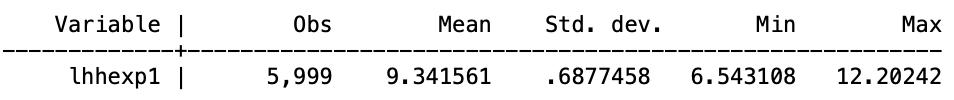
\includegraphics[scale=0.7]{Image_9/1.png}\\
    \textcolor{Magenta}{ci means lhhexp1}\\
    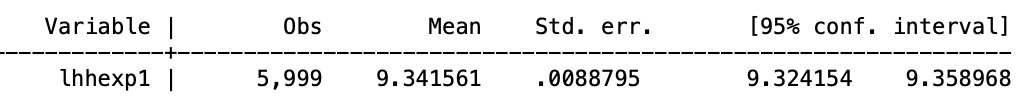
\includegraphics[scale=0.7]{Image_9/2.png}\\
    The 95\% confidence interval is [9.324154, 9.358968]\\

    \textbf{ii. Standard asymptotic theory using the boostrap mean and the boostrap standard errors}\\

    \solution\\

    \textcolor{Magenta}{bootstrap r(mean), reps(499): sum lhhexp1}\\
    First generate bootstrap sample with 499 repetitions at the mean then showing the summary.\\
    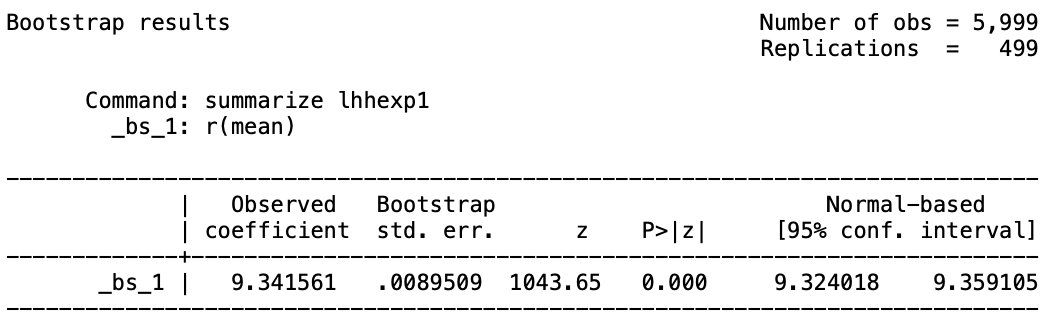
\includegraphics[scale=0.7]{Image_9/3.png}\\
    The 95\% confidence interval is [9.324018, 9.359105].\\

    \textbf{iii. The boostrap percentile method}\\

    \solution\\

    \textcolor{Magenta}{estat bootstrap, all}\\
    This is asking STATA to show the information of all bootstrap confidence interval construction methods.
    The middle line is the bootstrap confidence interval using the percentile method.\\
    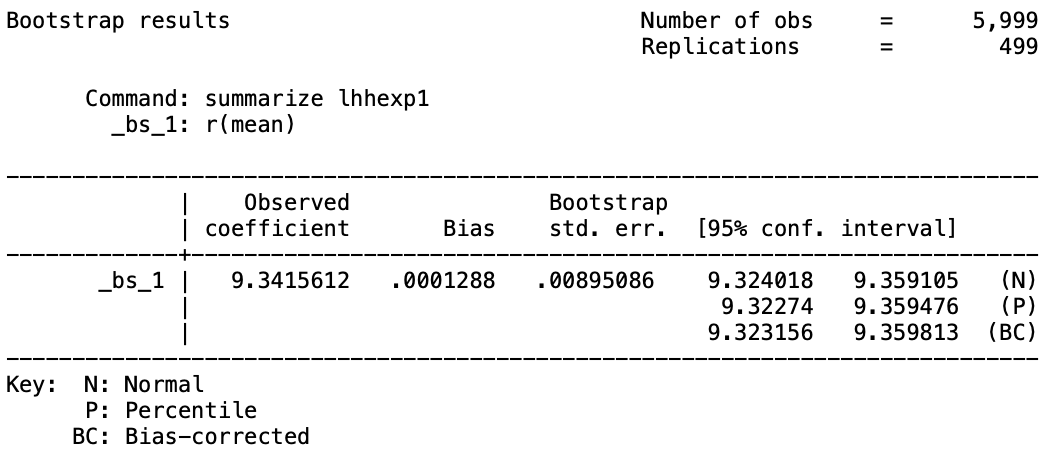
\includegraphics[scale=0.7]{Image_9/4.png}\\
    The 95\% confidence interval is [9.32274, 9.359476]\\

    \textbf{iv. The boostrap t-statistics with both methods}\\

    \solution\\

    Minimizing $S(b) = \frac{1}{N}\sum_{i=1}^{N}(Y-b)^2 \rightarrow$ taking the derivative and setting to zero
    \begin{gather*}
        \frac{2}{N}\sum_{i=1}^{N}(Y_i-\hat{b})=0\\
        \frac{2}{N}\sum_{i=1}^{N}Y_i - \frac{2}{N}\sum_{i=1}^{N}\hat{b} = 0\\
        \frac{2}{N}\sum_{i=1}^{N}Y_i - \frac{2}{N}N\hat{b} = 0\\
        2\hat{b} = 2\frac{1}{N}\sum_{i=1}^{N}Y_i\\
        \hat{b} = \frac{1}{N}\sum_{i=1}^{N}Y_i
    \end{gather*}
    which is just the sample mean.\\

    The first method is the \textbf{non-symmetric test} with the critical values of 
    $cv_{boot}(\frac{\alpha}{2})$ and $cv_{boot}(1-\frac{\alpha}{2})$ for $(\hat{t}_1,\ldots,\hat{t}_B)$.\\

    The second method is the \textbf{symmetric test} with the critical value of $cv_{boot}^a(1-\alpha)$
    for $(|\hat{t}_1|,\ldots,|\hat{t}_B|)$.

\end{homeworkProblem}

\begin{homeworkProblem}
    
    Suppose $X_1,\ldots, X_n$ are i.i.d. continuous r.v. from distribution with cumulative distribution function
    $F_X(\cdot)$ and probability density function $f_X(\cdot)$. Let $M_n$ be the \textbf{sample median} and $m_0$
    be the \textbf{population median}. 
    In this case $\displaystyle\sqrt{n}(M_n-m_0)\xrightarrow{d} N\left(0,\frac{1}{4(f_X(m_0))^2}\right)$.\\

    \textbf{i. Propose a consistent estimator for the asymptotic variance of $\sqrt{n}(M_n-m_0)$}\\

    \solution\\

    A consistent estimator for the density is $\displaystyle\frac{1}{4\hat{f}_x^2(M_N)}$ 
    where $\displaystyle\hat{f}_x(M_N) = \frac{1}{Nh}\sum_{i=1}^{N}K\left(\frac{y_i-M_N}{h}\right)$,
    a kernal density estimator.\\

    \textbf{ii. Obtain a 95\% CI for the median of lhhexp1}\\

    \textbf{A. using standard asymptotic theory with the consistent estimator proposed previously}\\

    \solution\\

    $SE(M_N) = \frac{1}{\sqrt{n}\sqrt{4f_X^2(M_N)}}$\\

    $(M_N - Z_{\frac{\alpha}{2}}\,SE(M_N), \,M_N + Z_{\frac{\alpha}{2}}\,SE(M_N))$\\

    $P(Z>Z_{\frac{\alpha}{2}}) = \frac{\alpha}{2},\,Z\sim N(0,1)$\\

    $h = 0.09904 \to$ obtained from Exercise sheet 8 with \textbf{Silverman's rule of thumb}\\

    Steps to do:
    \begin{enumerate}
        \item Find the median
        \item Generate the sequence
        \item Find the mean of sequence
    \end{enumerate}

    \textbf{B. using standard asymptotic theory with the bootstrap mean and bootstrap standard error}\\

    \solution\\

    \textbf{C. using the boostrap percentile method}\\

    \solution\\



\end{homeworkProblem}

\end{document}